\vspace*{4cm}
\begin{center}
\part{Mesh Benchmark Konzept und Testumgebung}\label{MeshBenchmarkKonzeptundTestumgebung}
\end{center}
\vspace*{\fill}
\clearpage

\section{Benchmark Konzept Mesh Netzwerke}\label{sec:BenchmarkKonzeptMeshNetzwerke}
Um die Performance der drei Mesh Stacks zu vergleichen wurde ein einheitliches Benchmark Konzept erarbeitet. Dieses definiert die Mesh Parameter, Testumgebungen, den Ablauf sowie sämtliche Messgrössen und Messreihen. Nachfolgend wird detailliert auf dieses Konzept eingegangen.

\subsection{Konzeptschema}\label{subsec:KonzeptschemaMesh}

Für den Vergleich der 3 Mesh Netzwerkstacks Bluetooth Mesh (BT Mesh), Thread und Zigbee wird ein vom Mesh Protokoll unabhängiges Testkonzept umgesetzt welches in der Abbildung \ref{fig:MeshTestKonzept} als Konzeptschema dargestellt ist.
Die Benchmark Slave Nodes (BSN) in der Abbildung als Sensoren und Aktoren mit unterschiedlichen Funktionalitäten dargestellt, bilden zusammen mit dem Benchmark Master Node (BMN) das zu testende Mesh Netzwerk.
\textit{Innerhalb des Netzwerks wird dessen Organisation vom jeweiligen Protokoll sichergestellt.} \todo[inline]{Raffi:  Das Benchamrk Managment wird nicht mehr vom Network Stack organisiert? }
Das Testnetzwerk soll ein realitätsnahes Netzwerk nachbilden.
Beispielsweise wird eine Hausautomation in einem Einfamilienhaus als Referenz angenommen in welchem jeweils nur gewisse Nodes untereinander Applikationsdaten austauschen.
Ein Lichtschalter kommuniziert nur mit einer Lichtquelle und umgekehrt. \todo[inline]{Raffi:  Es können auch mehrere Lampen sein? }
Der selbe Lichtschalter tauscht jedoch keine Applikationsdaten mit dem Temperatursensor aus.
Diese unterschiedlichen Beziehungen innerhalb des Mesh Netzwerks sind in der Abbildung \ref{fig:MeshTestKonzept} bereits angedeutet und werden im Abschnitt \ref{subsubsec:MeshBeziehungen} noch genauer beschrieben.

\begin{figure}[h]
	\centering
	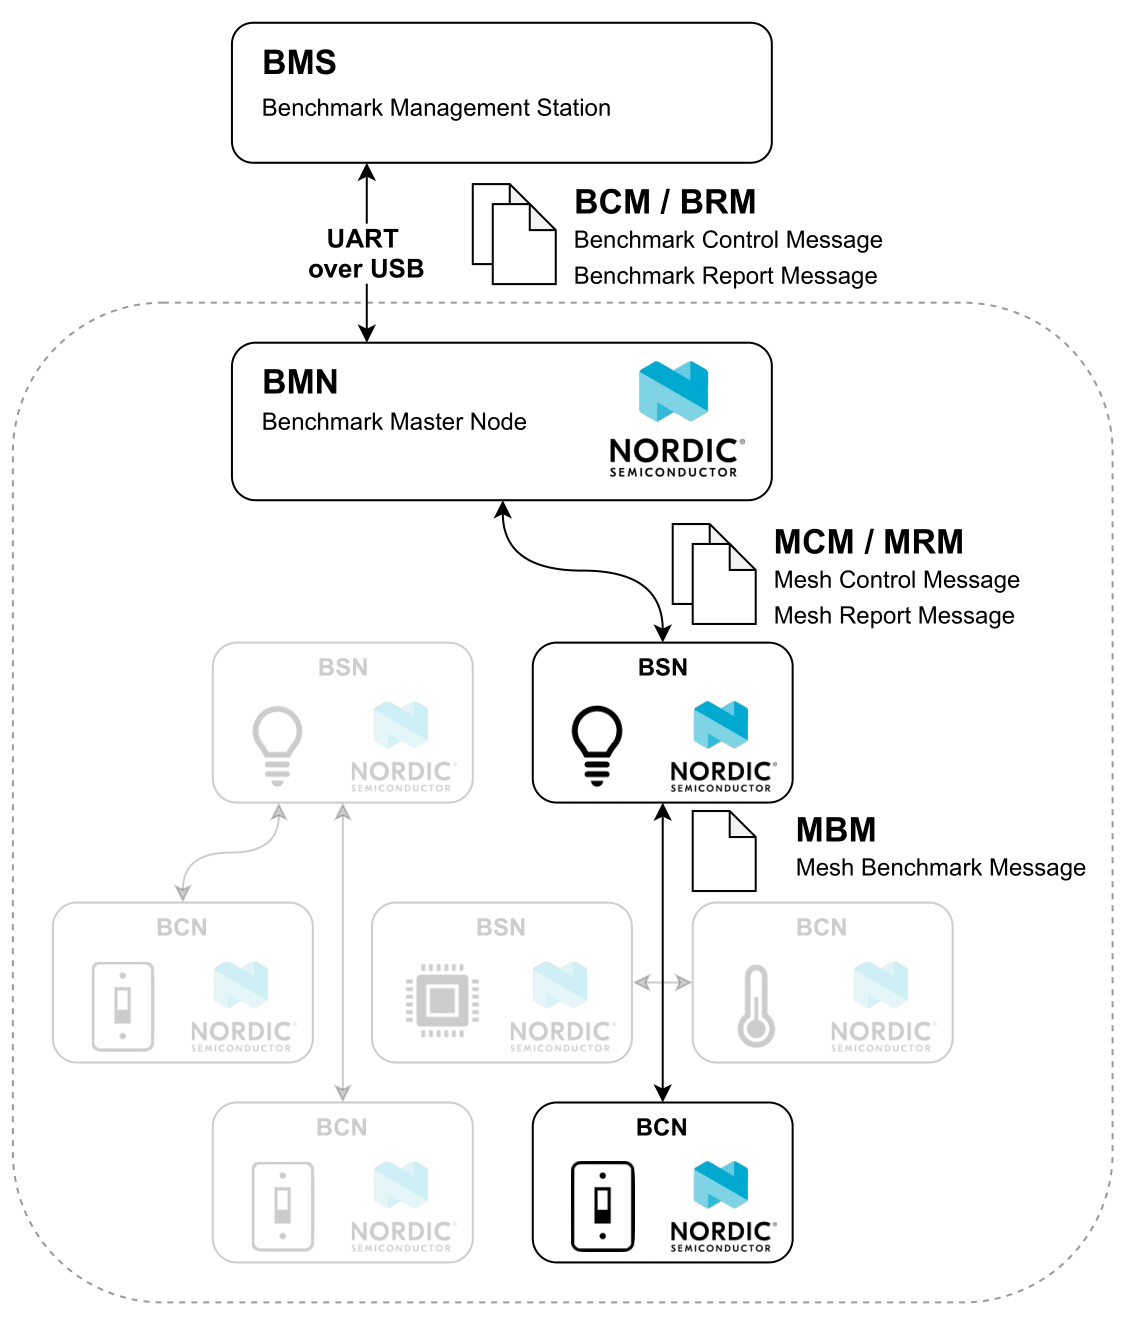
\includegraphics[width=0.6\textwidth]{Mesh_Testkonzeptschema.png}
	\caption{Konzeptschema für den Ablauf eines Mesh Benchmarks.}\label{fig:MeshTestKonzept}
\end{figure}

Die Benchmark Management Station (BMS) welche mit dem BMN via USB/UART kommuniziert, ist zuständig für die Verwaltung und Verarbeitung der Benchmarks. Während eines Benchmark Prozesses sollen sämtliche Messungen jedoch unabhängig von der BMS durchgeführt werden damit allfällige Latenzzeiten der USB/UART Verbindung die Resultate nicht verfälschen.

\subsubsection{Messages}\label{subsubsec:Messages}
In der Abbildung \ref{fig:MeshTestKonzept} sind verschiedene Messages dargestellt. Dabei handelt es sich um die Nachrichten die zwischen den einzelnen Teilen des Testaufbaus versendet werden und schliesslich einen Benchmark ausmachen. Die Messages besitzen Funktionen:

\paragraph{Mesh Benchmark Message (MBM)}
Die MBM ist jene Message welche die eigentlichen Messdaten produziert und diese sogleich unter den BSN (Mesh Knoten) überträgt. Anhand dieser Messages werden die Parameter für den Vergleich der Protokolle gemäss Abschnitt \ref{subsec:VergleichswerteundMessgrössenMesh} erfasst. Bei den MBM handelt es sich also um eine Sammlung von Messages welche je nach gewünschtem Messwert in Form und Anzahl unterschiedlich ausfallen können.

\paragraph{Mesh Control Message (MCM)}
Die MCM beinhaltet die Parameter für die Benchmarks welche vom BMN an alle BSN übertragen werden. Ausserdem werden damit Kontrollbefehle für die Benchmarks wie beispielsweise \textit{Start/Stop} sowie \textit{Laufzeit, Wiederholrate usw.} übertragen.

\paragraph{Mesh Report Message (MRM)}
Die MRM ist jene Message welche die Messwerte von den BSN an den BMN übertragen. Gleichzeitig wird damit auch gleich signalisiert, dass die Messung abgeschlossen wurde und mögliche Fehler oder sonstige Status übermittelt.

\paragraph{Benchmark Control Message (BCM)}
Die BCM beschreibt die Nachrichten welche zur Steuerung eines Benchmarks von der BMS her dienen. Dabei handelt es sich um Befehle wie beispielsweise \textit{Start/Stop}. Die BCM werden via serieller USB-UART Schnittstelle von der BMS zum BMN übertragen.

\paragraph{Benchmark Report Message (BRM)}
Die BRM beschreiben Nachrichten welche den Status oder die Ergebnisse eines Benchmarks aus dem Mesh zurück an die BMS melden. Sie werden vom BMN initiiert und gelangen über eine die selbe USB-UART Schnittstelle wie die BCM zum BMS. Die BRM wird erst nach Abschluss des Benchmarks initiiert. Zuvor werden die Messdaten auf dem BMN zwischen gespeichert.


\subsubsection{Nodes}\label{subsubsec:Nodes}
Wie bereits angedeutet und in Abbildung \ref{fig:MeshTestKonzept} gezeigt, kann im Mesh Benchmark zwischen den folgenden 3 Node Typen unterschieden werden.

\paragraph{Benchmark Master Node (BMN)}
Der Benchmark Master Node bildet den zentralen Zugriffspunkt zum Mesh Netzwerk für den Benchmark. Über ihn werden Control und Report Messages versendet und empfangen. Je nach Mesh Protokoll fungiert er zugleich als Mesh Leader (Thread) respektive Coordinator (Zigbee).

\paragraph{Benchmark Client Node (BCN)}
Der Benchmark Client Node repräsentiert beispielsweise einen Schalter in einer Lichtsteuerung. Im Benchmark Kontext ist er jene Instanz die MBM versendet.

\paragraph{Benchmark Server Node (BSN)}
Das Pendant zum BCN stellt der BSN dar. Er steht beispielsweise für eine Lichtquelle. Im Benchmark Kontext empfängt er die MBM die vom BCN versendet werden.


\subsection{Testszenarien}\label{subsec:TestszenarienMesh}

Die Benchmarks der Mesh Protokolle sollen mit unterschiedlichen Bedingungen getestet werden wobei grundsätzlich eine reelle Anwendung nachgebaut werden soll. Zum einen gibt es unterschiedliche Beziehungen innerhalb des Mesh Netzwerks, zum anderen werden Testumgebungen unterschieden.

\subsubsection{Mesh Beziehungen}\label{subsubsec:MeshBeziehungen}

\todo[inline]{Raffi:  Ist diese Information Relevant für das verständniss des Benchmarks?}

Innerhalb eines Mesh Netzwerks können 4 Beziehungen zwischen den Nodes für die Benchmarks unterschieden werden. Üblicherweise kommen mehrere oder sogar alle 4 Beziehungen innerhalb eines Netzwerkes gleichzeitig zum Einsatz. Abbildung \ref{fig:MeshTestBeziehungen} zeigt die Beziehungen.

\begin{itemize}
 	\item \textcolor{red}{Rot} stellt eine einfache P2P Verbindung ohne Hop dar. Beispielweise schaltet ein einzelner Schalter eine einzelne, definierte Lichtquelle
 	\item \textcolor{orange}{Orange} ist eine many-to-one Verbindung in welcher mehrere Lichtschalter die selbe Lichtquelle schalten.
 	\item \textcolor{cyan}{Blau} ist eine klassiche one-to-many Topologie dargestellt in welcher beispielsweise ein Schalter mehrere Lichtquellen bedient.
 	 \item \textcolor{green}{Grün} dargestellt ist eine indirekte P2P Verbindung mit. Das bedeutet, dass Schalter und Lichtquelle keine direkte Verbindung zueinander haben und daher Mesh-typisch via einem oder mehreren Hops kommuniziert.
\end{itemize}


\begin{figure}[H]
	\centering
	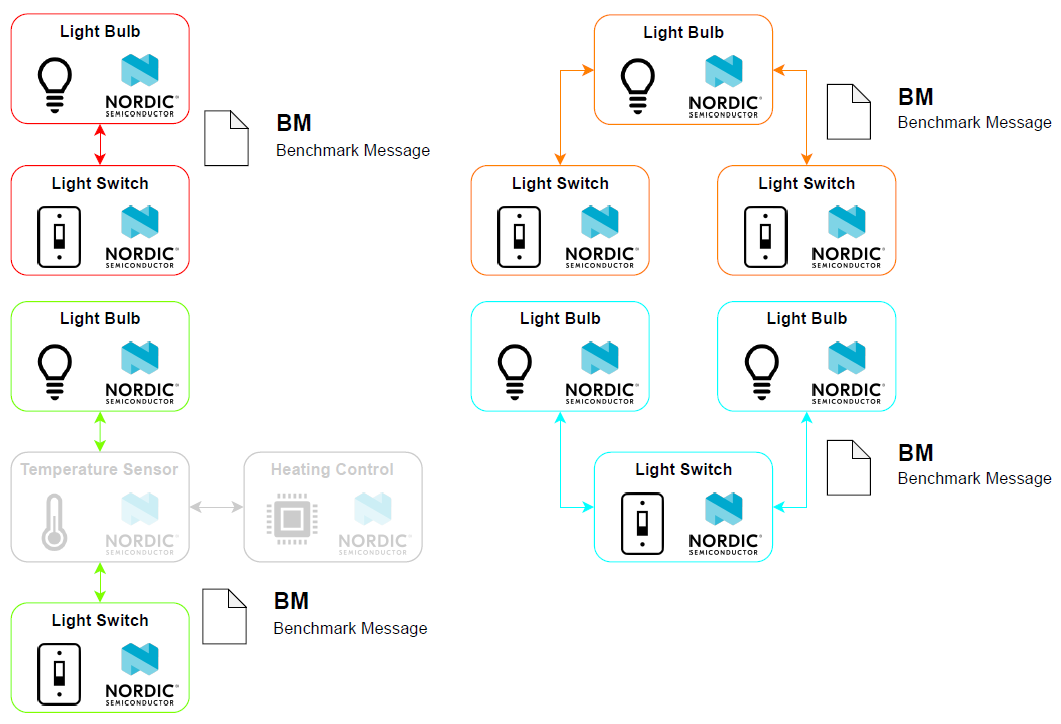
\includegraphics[width=1.0\textwidth]{Mesh_Test_Beziehungen.png}
	\caption{Beziehungen zwischen den Mesh Nodes innerhalb eines Benchmarks.}\label{fig:MeshTestBeziehungen}
\end{figure}


\subsubsection{Testumgebungen und Messaufbau}\label{subsubsec:TestumgebungenundMessaufbau}

Unterschiedliche Testumgebungen sollen die Benchmarks und schlussendlich den Vergleich der 3 Mesh Protokolle aussagekräftiger machen.
Nachfolgende Umgebungen mit den entsprechenden Eigenschaften sollen getestet werden.
Die Abbildungen zu den Testumgebungen zeigen jeweils die Platzierung der Nodes sowie deren Funktion und Gruppen Zugehörigkeit. Die Farbe Grün identifiziert den Node als Client Node während Blau für einen Server Nodes steht. Die Nummerierung zeigt welcher Node zu welcher Adressgruppe gehört. Ein Client Node in Gruppe 1 sendet jeweils Nachrichten zu allen Server Nodes in der selben Gruppe.

\paragraph{Labor}
Der Laboraufbau ist ein Extremtest welcher die Leistungsgrenzen der Protokollstacks ausloten soll. Dabei werden die Nodes auf einem Raster gemäss Abbildung \ref{fig:AnordnungLaborTestumgebungMessumgebung1} angeordnet. Die genauen Abmessungen sind der Abbildung zu entnehmen.
\begin{itemize}
	\item Testaufbau unter Laborbedingungen auf engstem Raum.
	\item Ausgeglichene Anzahl Sensoren und Aktoren.
	\item Sehr Hohe Node-Dichte.
	\item Geringe bis keine Störbeeinflussung durch die Umgebung zu  erwarten.
	\item Die Mesh-Beziehungen werden künstlich bestimmt sodass einfache P2P Verbindungen mit oder ohne Hop entstehen.
\end{itemize}


\begin{figure}[H]
\centering
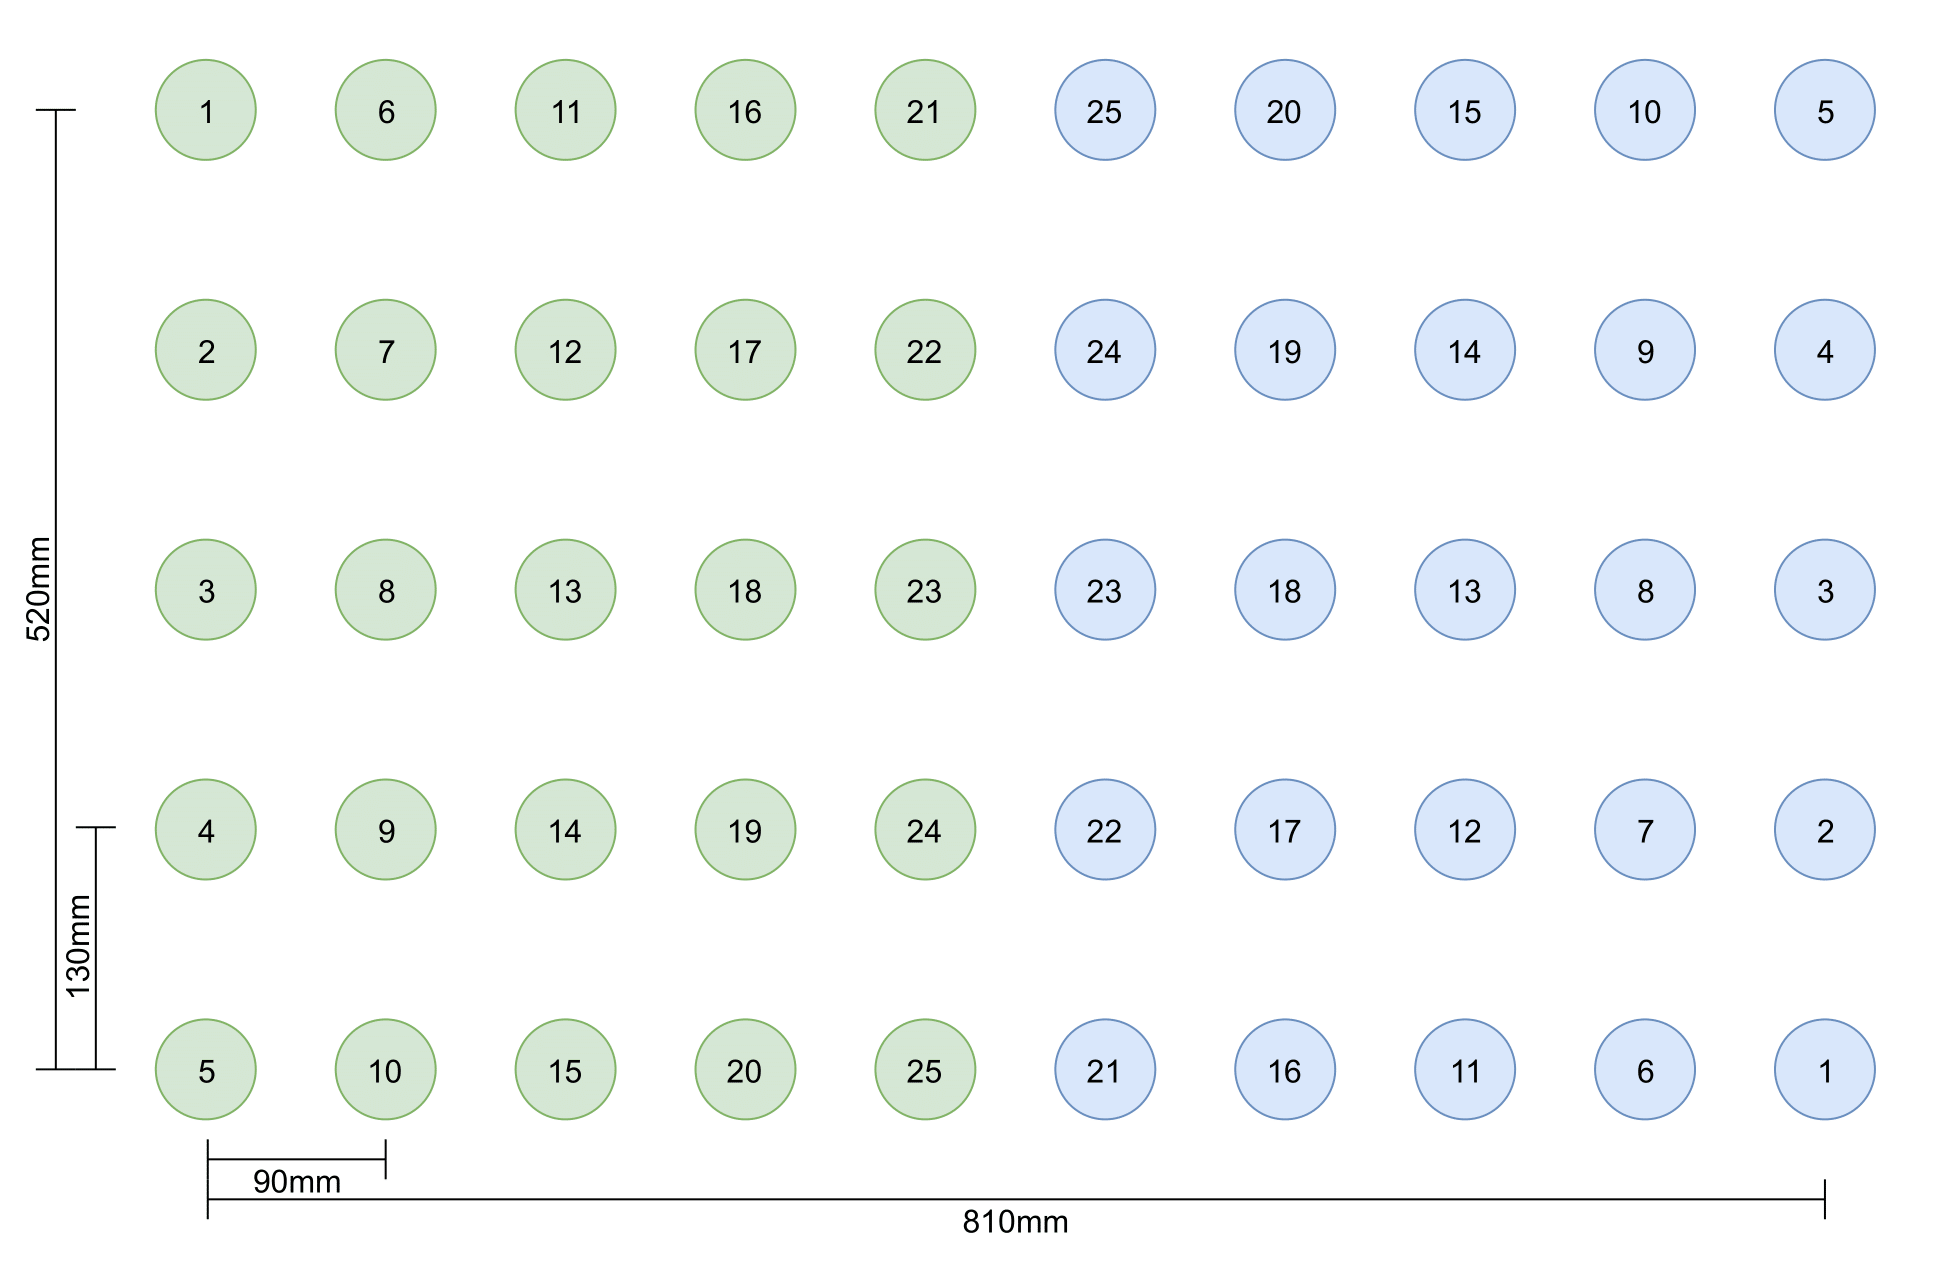
\includegraphics[width=0.7\textwidth]{Testaufbau_Labor.png}
\caption{Anordnung Labor Testumgebung, Messumgebung 1}\label{fig:AnordnungLaborTestumgebungMessumgebung1}
\end{figure}

\paragraph{Einfamilienhaus}
Die Testgeräte werden in einem Einfamilienhaus installiert und repräsentieren damit eine flächendeckende Heim-Automatisierung. Folgende Eingenschaften soll diese Messung abdecken:
\begin{itemize}
	\item Einfamilienhaus über mehrere Etagen.
	\item Node-Dichte relativ gering.
	\item Kleine Beeinflussung durch Nachbarsysteme sind zu erwarten.
	\item Sämtliche Mesh-Beziehungen gemäss \ref{subsubsec:MeshBeziehungen} kommen vor und werden durch die bestehende Infrastruktur bestimmt.
\end{itemize}

Die Abbildung \ref{fig:Messumgebung2Einfamilienhaus} zeigt die Platzierung der Nodes auf den 4 Etagen des Einfamilienhauses.

\begin{figure}[H]
	\centering
	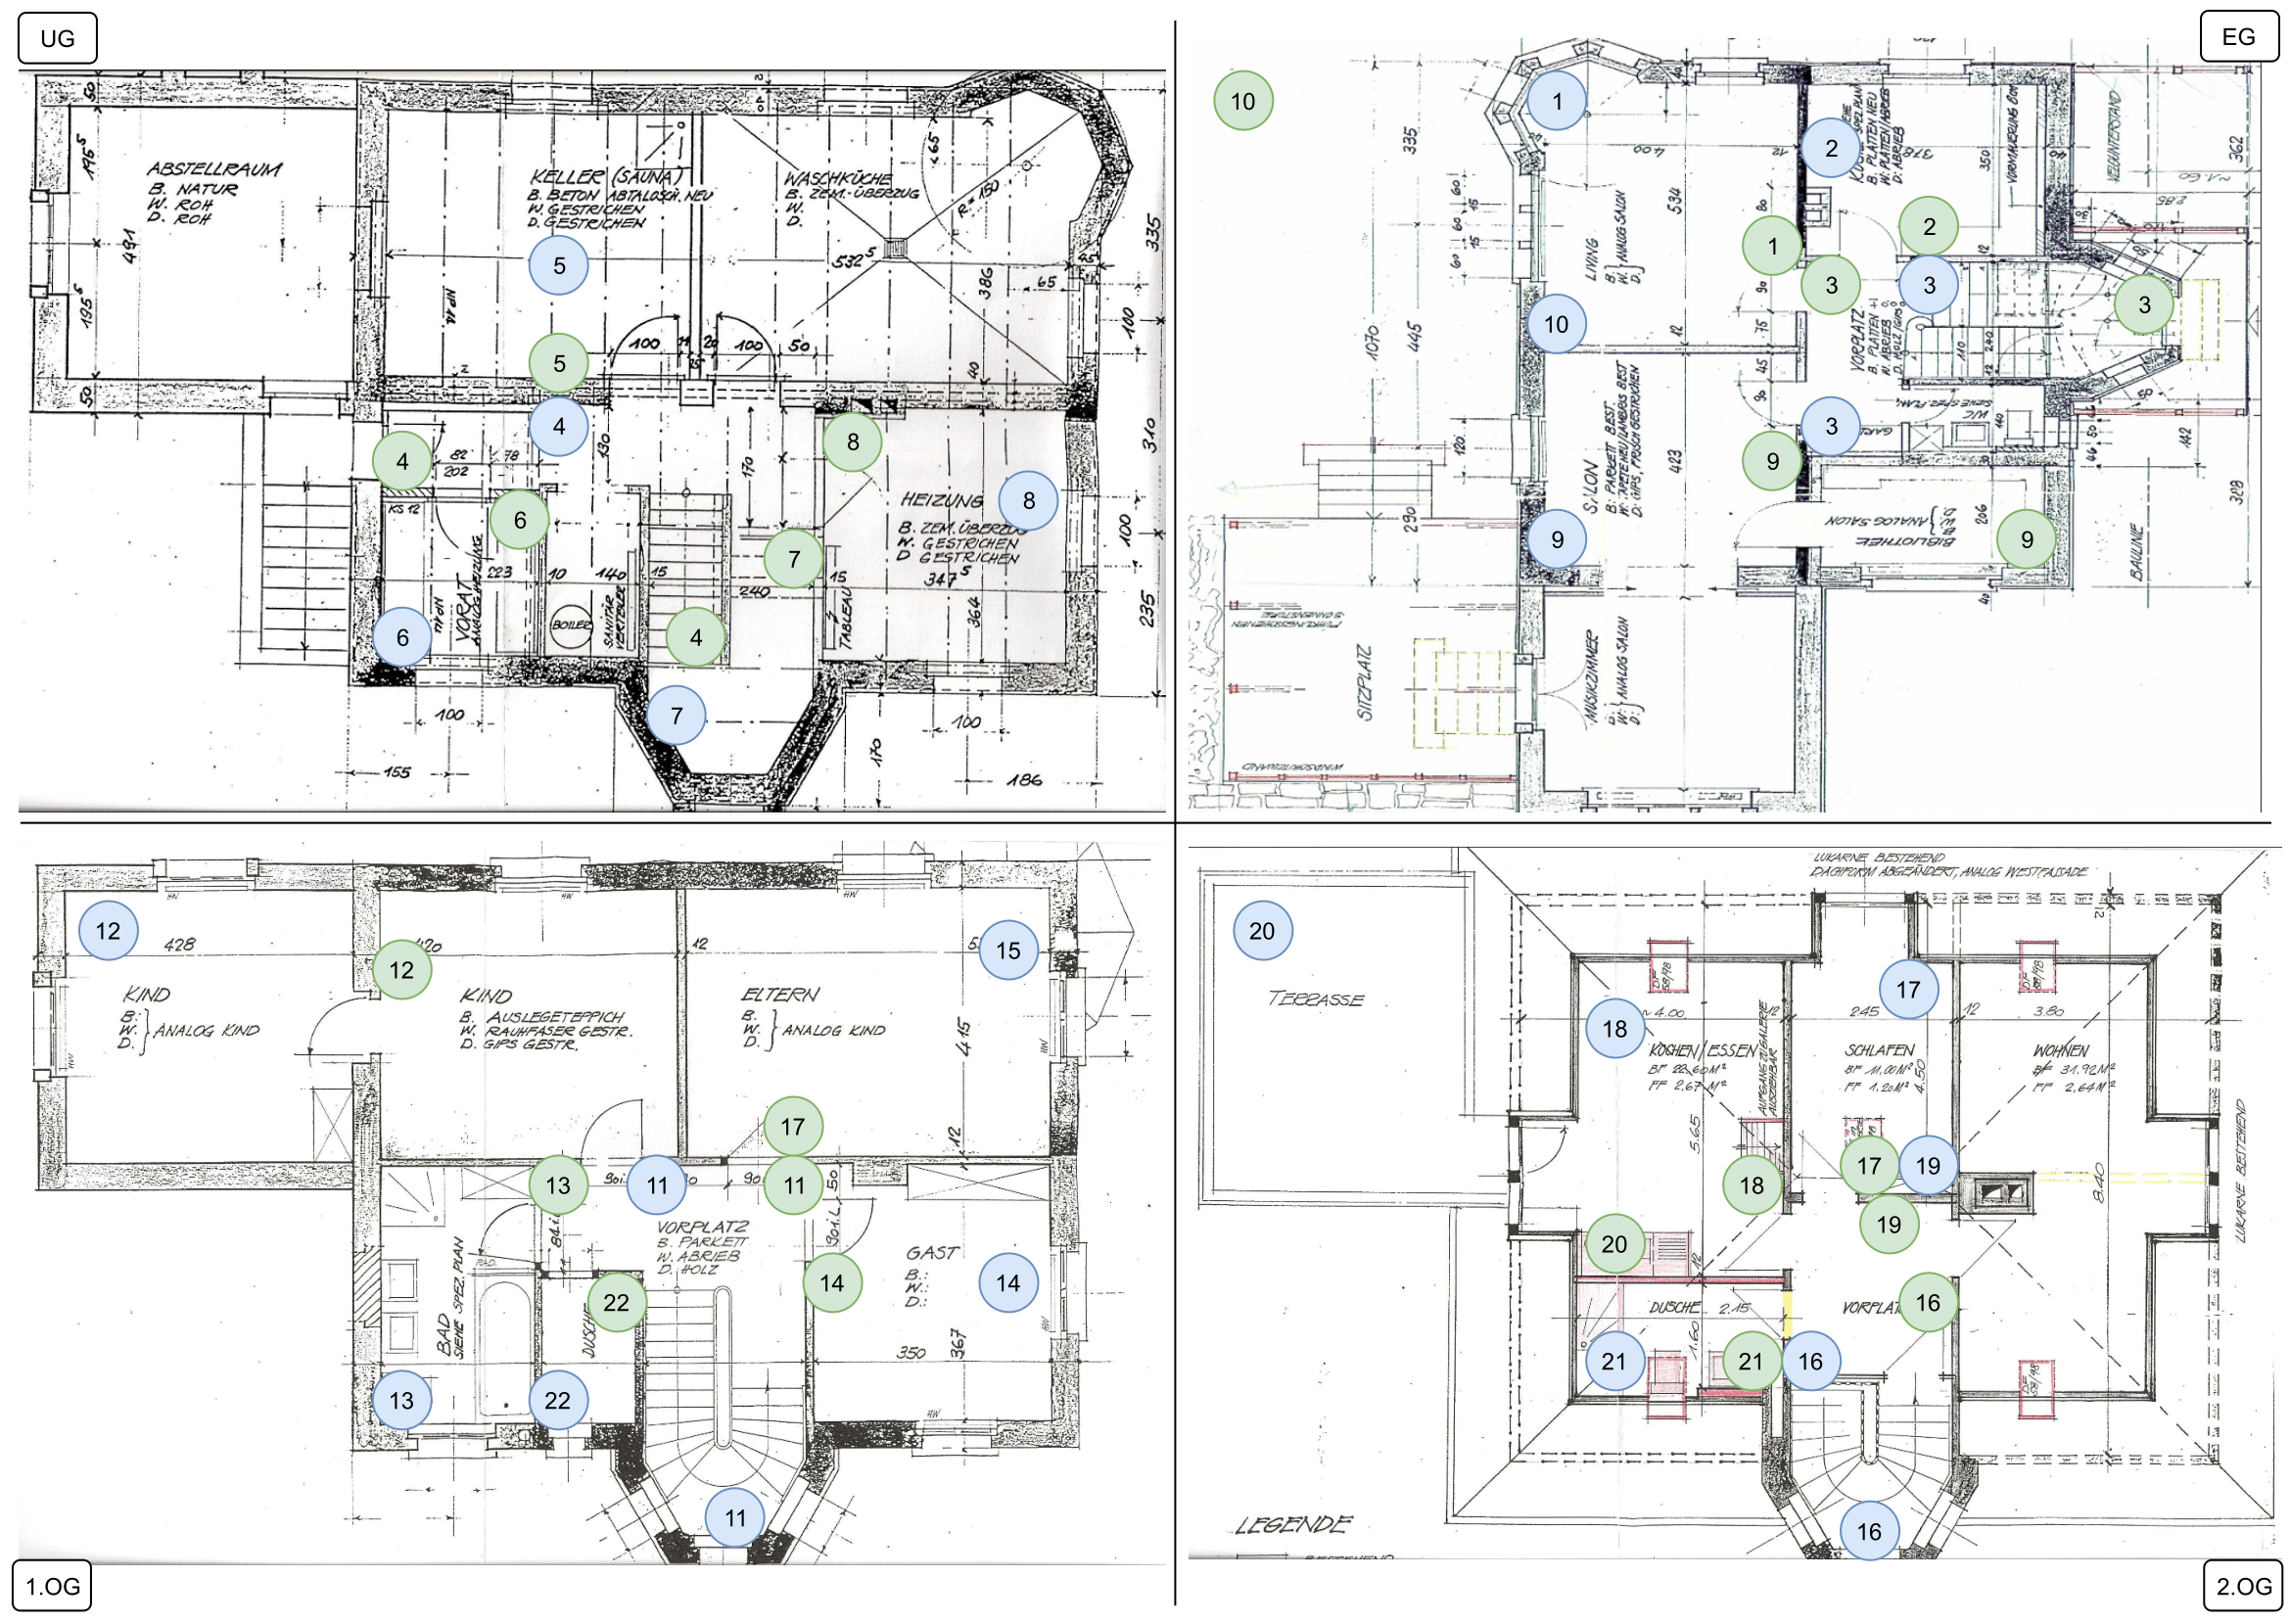
\includegraphics[width=\textwidth]{Plan_Haus_Raffi.png}
	\caption{Platzierung der Nodes im Einfamilienhaus}\label{fig:Messumgebung2Einfamilienhaus}
\end{figure}
	
\paragraph{Wohnung}
Ebenfalls als Heim-Automatisierung gedacht werden die Messungen in einer Wohnung durchgeführt.
\begin{itemize}
	\item Wohnung über eine Etage in einem Mehrfamilienhaus
	\item Anzahl Sensoren und Aktoren vergleichbar gross.
	\item Node-Dichte höher als im Haus.
	\item Mögliche Störeinflüsse durch andere Systeme von Nachbarn sind zu erwarten.
	\item Sämtliche Mesh-Beziehungen gemäss \ref{subsubsec:MeshBeziehungen} kommen vor und werden durch die bestehende Infrastruktur bestimmt.
\end{itemize}

Bei der Wohnung handelt es sich um eine 3.5 Zimmer Wohnung mit einer Wohnfläche von 122 Quadratmetern. Die genauen Abmessungen sowie die Platzierung der Nodes ist in Abbildung \ref{fig:PlatzierungderNodesinMessumgebung3} zu sehen.

\begin{figure}[H]
	\centering
	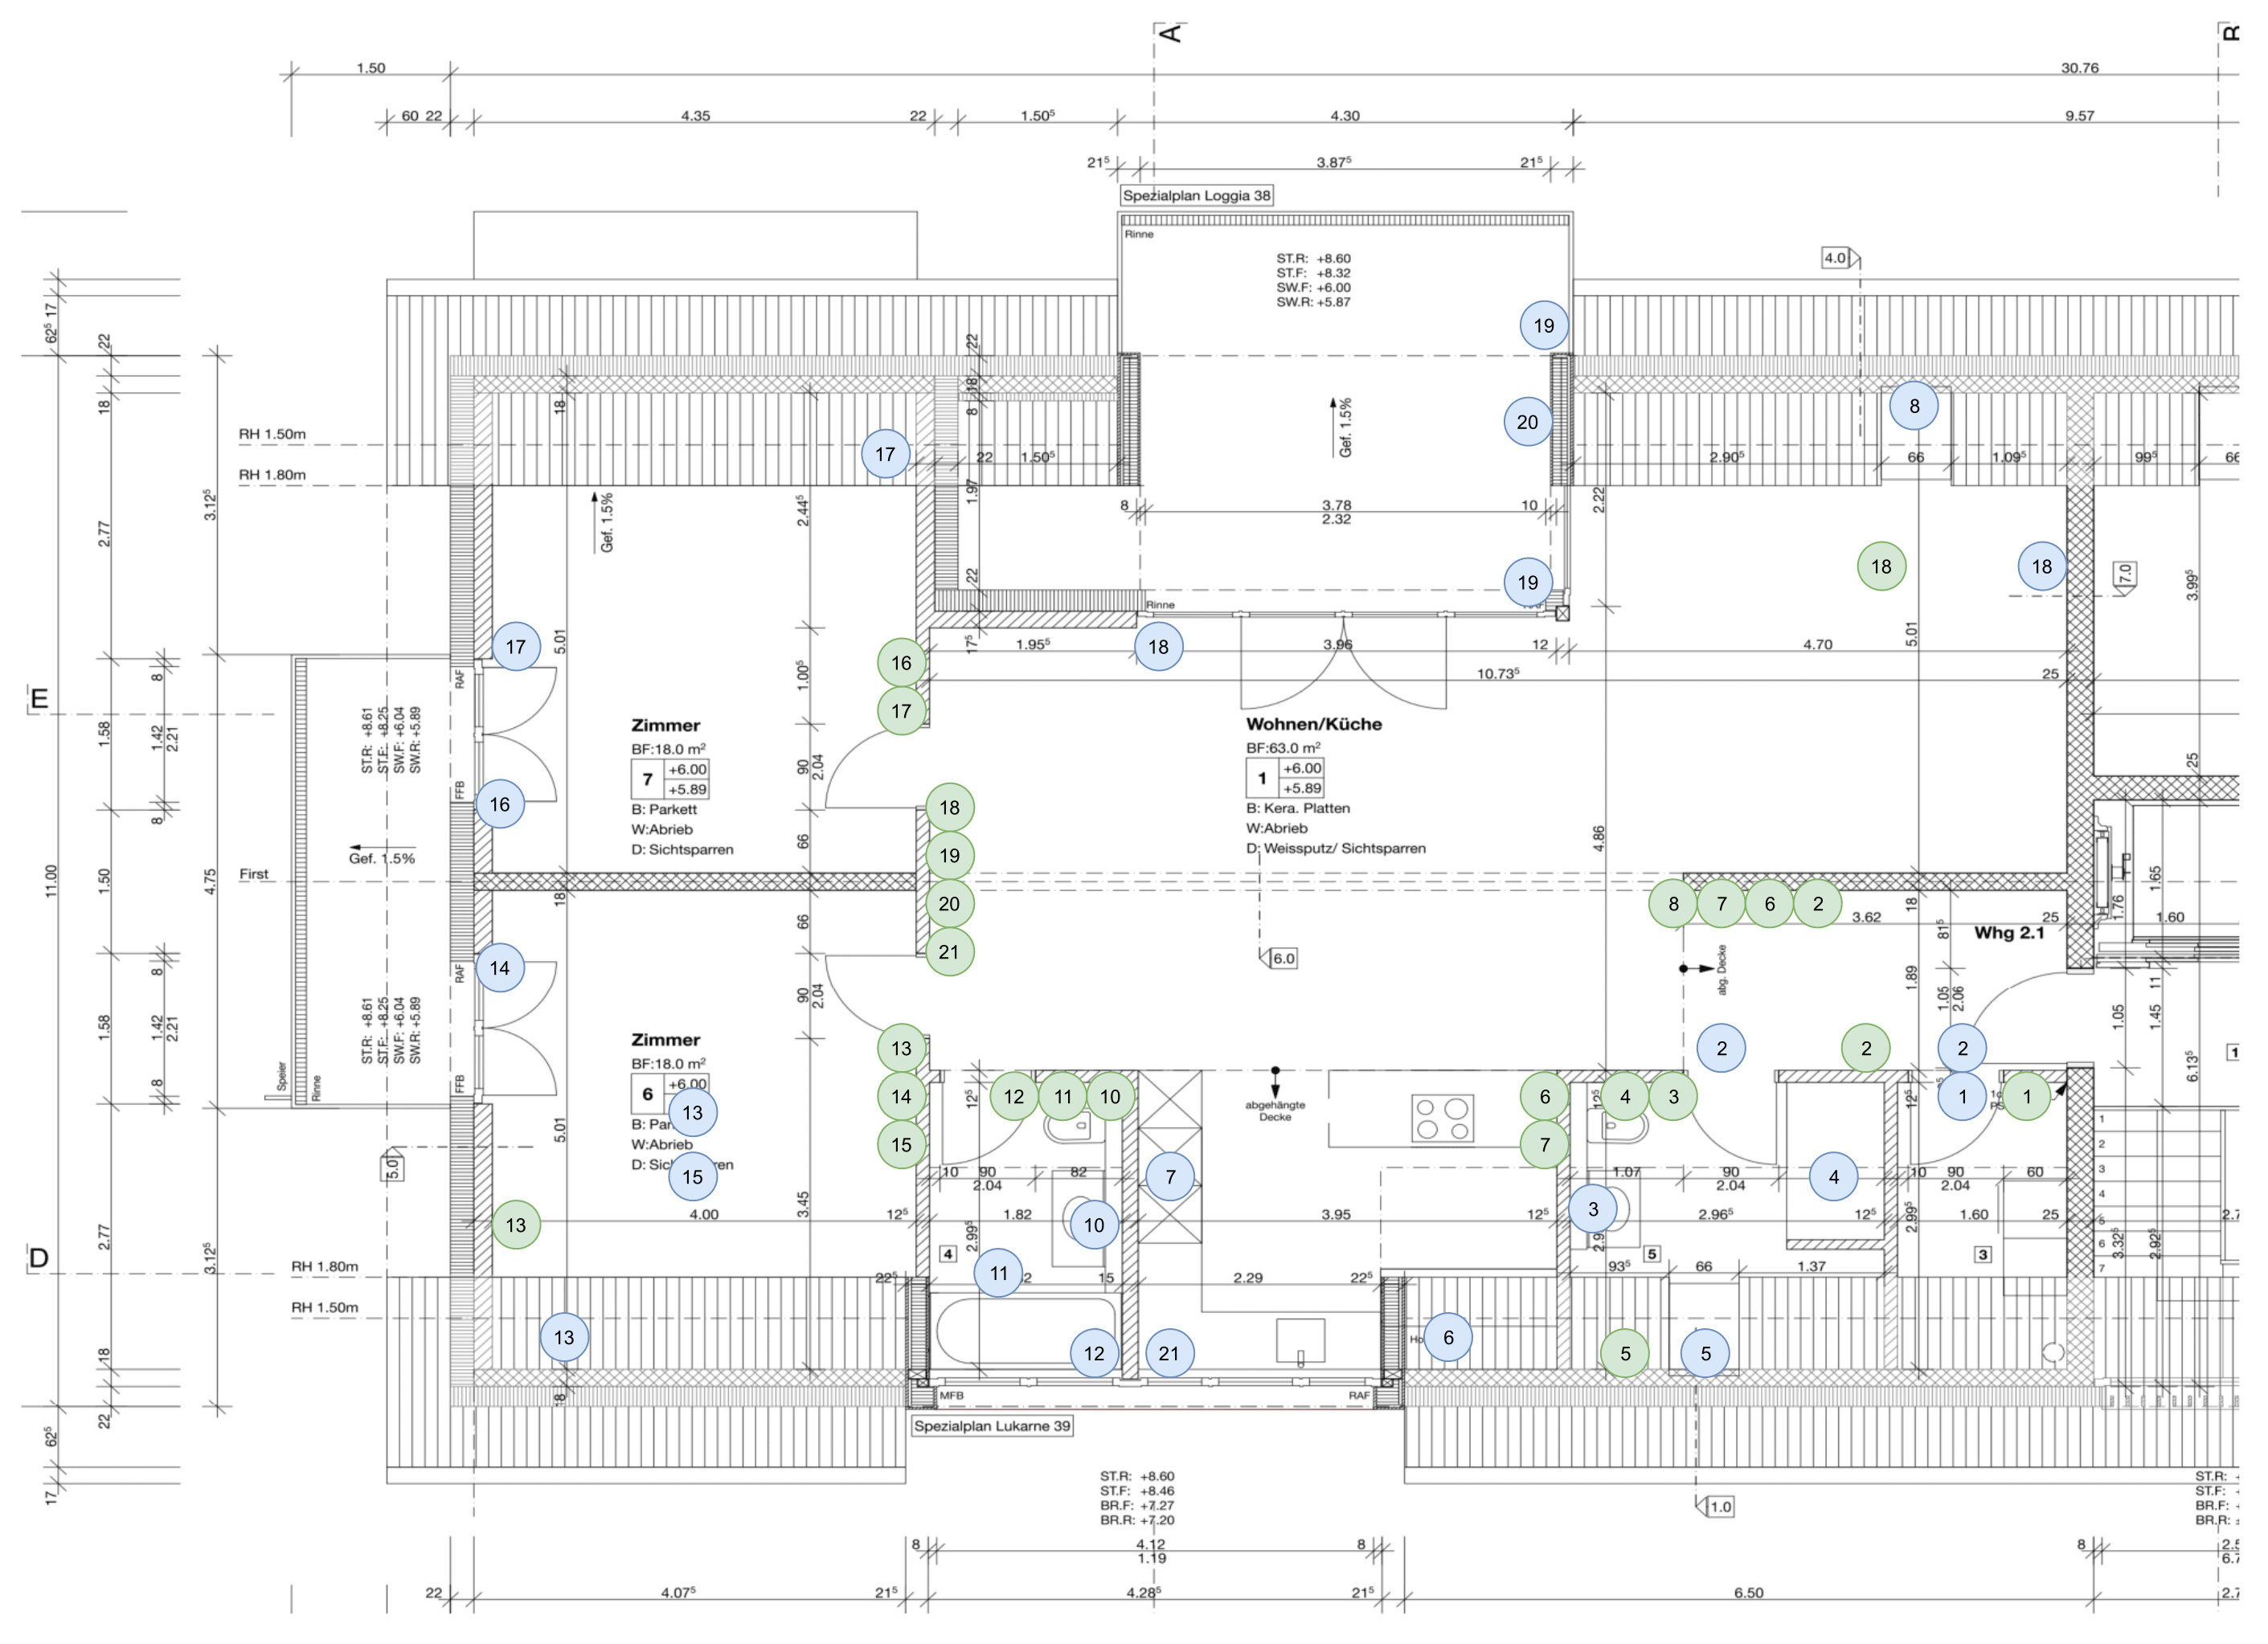
\includegraphics[width=\textwidth]{Plan_Wohnung_Cyrill_Nodes_Placement.png}
	\caption{Platzierung der Nodes in Messumgebung 3 (Wohnung)}\label{fig:PlatzierungderNodesinMessumgebung3}
\end{figure}




\subsection{Ablauf}\label{subsec:AblaufMesh}

Ein Mesh Benchmark folgt einem klar definierten Ablauf. Die Abbildung \ref{fig:MeshTestKonzept} zeigt das Testkonzept in welchem auch der Ablauf eines Benchmarks bereits angedeutet ist.

\begin{enumerate}
	\item \textbf{Benchmark User-Init:}\\
	Im Config File auf dem BMS werden die gewünschten Parameter definiert, die Konfiguration verteilt und der Benchmark durch den Benutzer gestartet.
	\item \textbf{Benchmark Init BMN:}\\
	Die Parameter werden an den BMN übergeben welcher diese wiederum an alle teilnehmenden BSN weiterleitet. Mit einem Startsignal vom BMN wird der Benchmark auf den BSN gestartet.
	\item \textbf{Benchmark Prozess:}\\
	Die BSN führen den Benchmark Prozess mit den definierten Parametern aus. Dies geschieht autonom und jeweils nur zwischen den entsprechenden BSN die gemäss Benutzerkonfiguration in einer direkten Beziehung zueinander stehen (siehe Mesh Beziehungen \ref{subsubsec:MeshBeziehungen}). Die entstandenen Messdaten werden auf den BSN zwischengespeichert und nach Ablauf des Benchmarks ins Flash geschrieben.
	\item \textbf{Reporting:}\\
	Nach Ablauf der Benchmark Zeit werden die Messdaten an den BMN übertragen. Dies erfolgt gesteuert durch den BMN welcher die Daten bei einem BSN nach dem anderen abfragt und direkt an das BMS weiterleitet.
	\item \textbf{Finish:}\\
	Der BMN kontrolliert ob er die Daten von sämtlichen BSN korrekt auslesen konnte und bestätigt das Ende der Messung gegenüber dem BMS.
	\item \textbf{Auswertung:}\\
	Das BMS beendet den Benchmark Vorgang, speichert die Messdaten in seiner Datenbank ab und bereitet diese grafisch auf. 
\end{enumerate}

%\subsection{Anforderungen}\label{subsec:SoftwareAnforderungen}
%\todo[inline]{Titel ändern. Und Text an restliches Kapitel anpassen.}
%Wie bereits im Abschnitt \ref{sec:Abgrenzung} wurden die Anforderungen in der Aufgabenstellung (siehe Anhang \ref{app:Aufgabenstellung}) sowie im Pflichtenheft (siehe Anhang \ref{app:Pflichtenheft}) vorgängig festgelegt. Im Fokus steht das erfassen der wichtigsten Messgrössen welche nachfolgend aufgeführt werden.
%
%\begin{itemize}
%	\item \textbf{Latenzzeit}: Bestimmung der Latenzzeit in Millisekunden zwischen den Teilnehmern. Die Genauigkeit sollte bei $+/-$1 ms liegen.  
%	\item \textbf{Anzahl Hops}: Bestimmung der Anzahl Hops, über welche eine Nachricht übermittelt wird.
%	\item \textbf{Datenrate}: Messen der Datenrate in Bytes/s, welche zwischen zwei Teilnehmern erreicht wurde. 
%	\item \textbf{RSSI}: Erfassen des RSSI-Werts der eingehenden Pakete.
%	\item \textbf{Paketverlust}: Pakete zählen, welche ihr Ziel nicht erreicht haben.  
%	\item \textbf{Aktive Radio Zeit}: Erfassen der aktiven Radio-Zeit um den Energieverbrauch abschätzen zu können. 
%\end{itemize}
%
%
%Die Erfassung muss in allen Mesh-Netzwerken möglich sein. Um die Messresultate vergleichen zu können müssen die gleichen Ausgangslagen vorliegen, sowie die selben Messmethoden angewendet werden. 



\subsection{Vergleichswerte und Messgrössen}\label{subsec:VergleichswerteundMessgrössenMesh}
Beim Vergleich der Mesh Protokolle wird zwischen Vergleichswerten und Messgrössen unterschieden. Vergleichswerte sind meist aus einer oder mehreren Messgrössen berechnete Werte die einen aussagekräftigen Vergleich ermöglichen.

\subsubsection{Vergleichswerte}\label{subsubsec:Vergleichswerte}
Im Pflichtenheft zu dieser Arbeit (Anhang \ref{app:Pflichtenheft}) wurden die Testkriterien für den Vergleich bereits ausführlich behandelt.
Folgende Vergleichswerte kommen nun in der Auswertung effektiv zum Tragen:

\begin{itemize}
	\item \textbf{Latenzzeit}: Bestimmung der Latenzzeit in Millisekunden eines Pakets das über das Mesh vom Client zum Server versendet wird.  
	\item \textbf{Anzahl Hops}: Bestimmung der Anzahl Hops, über welche eine Nachricht übermittelt wird.
	\item \textbf{Datenrate}: Messen der Datenrate in Bytes/s, welche zwischen zwei Teilnehmern erreicht wurde. 
%	\item \textbf{RSSI}: Erfassen des RSSI-Werts der eingehenden Pakete.
	\item \textbf{Paketverlust}: Pakete welche ihr Ziel nicht erreichen konnten werden gezählt um so eine Paketverlustrate zu ermitteln.
	\item \textbf{Aktive Radio Zeit}: Zur Abschätzung des Energieverbrauchs der Nodes im Mesh Betrieb, wird die Aktivdauer der Radio Schnittstelle gemessen.
\end{itemize}


\subsubsection{Messgrössen}\label{subsubsec:Messgrössen}

Um diese Werte zu erfassen sind spezifische Messgrössen gefragt die auf den Nodes direkt erfasst werden können.
Die untenstehende Auflistung zeigt die auf den Mesh Nodes erfassten Messgrössen, deren Generierung und wie diese in der Auswertung verwendet werden.


\paragraph{Message Timestamp}
Zur Bestimmung der Latenzzeit eines Pakets das über das Mesh Netzwerk versendet wird, wird beim Senden sowie beim Empfangen ein Message Timestamp erfasst.
Die unter den Nodes synchronisierte Zeit gibt Aufschluss darüber wie lange das Paket unterwegs war. Die Berechnung der Latenzzeit wird jedoch erst bei der Analyse auf dem BMS durchgeführt.

\paragraph{Number of Hops}
Die oben erwähnte Latenzzeit ist in einem Mesh Netzwerk abhängig vom Weg den ein Paket bei der Übermittlung genommen hat. Mit jedem Hop nimmt die Latenzzeit zu.
Deshalb wird beim Server Node die Anzahl Hops die das Paket genommen hat aus dem Message Header ausgelesen und für die Bestimmung der Latenzzeit abgespeichert.

\paragraph{Source-, Destination-, Group-Address}
Aufgrund der veränderlichen Beziehungen von Client und Server Nodes ist die Zuordnung von Quell- und Zieladresse eines Pakets ebenfalls nicht statisch. Aus diesem Grund werden auf allen Nodes die Quell-, Ziel- und Gruppenadressen der Pakete ausgelesen. 
Somit kann das Benchmark Paket eindeutig identifiziert und in der Auswertung erfasst werden.
Die Adressinformationen werden aus dem Message Header des Mesh Pakets ausgelesen oder im Falle des Client Nodes mit der Benchmark Control Message übermittelt.

\paragraph{Message ID}
Als Payload im Mesh Paket versendet, identifiziert die Message ID das Paket zusammen mit den Adressinformationen eindeutig. So kann Paketverlust wie auch die Latenzzeit erfasst werden.

\paragraph{RSSI}
Der RSSI (Received Signal Strength Indication) wird auf dem Server Node auf MAC Ebene erfasst und zeigt die Empfangsstärke zum zuletzt passierten Hop. Dies gibt Aufschluss über die Empfangsqualität und kann bei der Analyse des Benchmarks als weiterer Indikator für Paketverlust und Latenzzeit verwendet werden.

\paragraph{Aktive Radio Zeit}
Die Zeit in der die Radio Schnittstelle aktiv ist wird auf dem Node direkt gestoppt und gespeichert.


\subsection{Messreihe}\label{subsec:Messreihe}
Um die Mesh Protokolle einem möglichst fairen Vergleich zu unterziehen, werden pro Testumgebung eine Reihe an Messungen durchgeführt. Die Tabelle \ref{tab:ParameterBenchmarkMessreihe} zeigt Total 8 Messreihen mit den entsprechenden Parametern.

\begin{table}[h]
\centering
\begin{adjustbox}{width=1\textwidth}
\begin{tabular}{|c|c|c|c|c|c|c|c|c|} 
\cline{2-9}
\multicolumn{1}{c|}{} & \multicolumn{5}{c|}{Benchmark Parameter} & \multicolumn{3}{c|}{Messaufbau} \\ 
\hline
\textbf{\#}  & \textbf{Msg. Gen.}  & \textbf{Duration} & \textbf{Msg. Cnt.}  & \textbf{Payload }  & \textbf{Disturbance}  & \textbf{Labor}  & \textbf{Haus}  & \textbf{Wohnung}  \\ 
\hline
1 & Rand & 600s & 60 & Small & No & x & x & x \\ 
\hline
2 & Seq & 600s & 60 & Small & No & x & x & x \\ 
\hline
3 & Rand & 600s & 60 & Large & No & x & x & x \\ 
\hline
4 & Seq & 600s & 60 & Large & No & x & x & x \\ 
\hline
5 & Rand & 600s & 600 & Small & No & x & x & x \\ 
\hline
\multicolumn{1}{c}{} & \multicolumn{1}{c}{} & \multicolumn{1}{c}{} & \multicolumn{1}{c}{} & \multicolumn{1}{c}{} & \multicolumn{1}{c}{} & \multicolumn{1}{c}{} & \multicolumn{1}{c}{} & \multicolumn{1}{c}{} \\ 
\hline
6 & Rand & 600s & 60 & Small & Yes & x &  &  \\ 
\hline
7 & Seq & 750s & 10 & Small & No & x &  &  \\ 
\hline
8 & Seq & 750s & 10 & Large & No & x &  &  \\
\hline
\end{tabular}
\end{adjustbox}
\caption{Parameter Benchmark Messreihe}
\label{tab:ParameterBenchmarkMessreihe}
\end{table}

Die Erläuterungen über die Bedeutung der Parameter ist in der folgenden Übersicht \ref{tab:BedeutungBenchmarkParameter} zu finden. 

\begin{table}[h]
\centering
\begin{adjustbox}{width=1\textwidth}
\begin{tabular}{lll} 
\toprule
Parameter: & Gültige Werte: & Bedeutung: \\ 
\hline
Msg. Gen & Seq/Rand & Nachrichten Generierung Sequentiell oder Pseudozufällig \ref{subsec:TrafficGeneration}. \\
Duration & Ganze Zahlen & Dauer eines Benchmarks angegeben in Sekunden. \\
Msg. Count & Ganze Zahlen & Anzahl der Nachrichten die pro Client Node versendet werden.\\
Payload & Small/Large & Grosse oder Kleine Payload gemäss Definition in Tabelle.\\
Disturbance & Yes/No & \begin{tabular}[t]{@{}l@{}}Gewollte Störung durch P2P Testinfrastruktur auf\\dem selben Channel. \end{tabular} \\
\bottomrule
\end{tabular}
\end{adjustbox}
\caption{Bedeutung Benchmark Parameter}
\label{tab:BedeutungBenchmarkParameter}
\end{table}

Die Messungen 1 bis 5 werden in allen drei Messaufbauten durchgeführt. So werden die Unterschiede der Topologien ersichtlich.
Die Messungen 6 bis 8 hingegen werden nur im Laboraufbau durchgeführt damit allfällige Externe Störeinflüsse ausgeschlossen werden können und das Mesh Netzwerk unter Extrembedingungen getestet werden kann.

Bei der Messung mit dem Index 6 handelt es sich um ein Benchmark welcher mit der P2P Testinfrastruktur gestört wird. So soll die Störimmunität des Mesh Stacks getestet werden.
Die Messungen 7 und 8 wurden aufgrund der Erfahrungen die mit den Resultaten der Messungen 1 bis 6 gesammelt werden konnten, nachträglich ergänzt. In Abschnitt \ref{sec:Validierung} wird genauer auf diese Problematik eingegangen.
Die Dichte der Nachrichten ist bei diesen Messungen deutlich tiefer.





\subsection{Allgemeine Benchmark Parameter}\label{subsec:AllgemeineBenchmarkParameter}

Die oben erwähnten Messreihen haben nebst den variablen Parametern einige allgemeingültige Benchmark Parameter die in der Tabelle \ref{tab:AllgemeineBenchmarkParameter} aufgeführt sind.
Diese sind für sämtliche Messungen innerhalb des jeweiligen Mesh Protokolls gültig.
Die ersten vier Parameter \textit{Group addressing mode, Application Layer, MAC Layer sowie Mesh Node Type} sind Protokoll abhängig und deshalb bei allen drei Mesh Stacks unterschiedlich.
Da sich diese Parameter innerhalb des jeweiligen Protokolls unterschiedlich umsetzen lassen sind die gewählten Werte resp. Funktionen hier aufgelistet.
Deren Funktionsweise wird in separaten Abschnitten noch detailliert behandelt.

\todo[inline]{Raffi: Verweis auf die jeweiligen Abschnitte? Oder den Letzte Satz weg lassen.} 

Beim \textit{Group addressing mode} wird zwischen Broadcast bei BT Mesh, Multicast bei Thread und Unicast bei Zigbee unterschieden. Gemäss Definition im Pflichtenheft soll jeweils eine Gruppenadressierung stattfinden. Zigbee bietet zwar eine solche Möglichkeit eines Multicasts jedoch wird dieser schliesslich als Broadcast umgesetzt was eine deutliche Limitierung der Performance verursacht.
Aufgrund dieser Erfahrung und der Erkenntnis dass marktübliche Lichtsteuerungen\footnote{Analyse mittels Sniffer Trace einer IKEA Tradfri Lichtsteuerung.} nur selten ein solches Multicast Prinzip verwenden, wird die Adressierung im Benchmark gerichtet (Unicast) vorgenommen (siehe auch \ref{sec:ZigbeeUmsetzungBenchmark}).
Das bedeutet die Nachrichten werden nicht an eine Gruppenadresse sondern direkt an die jeweilige Node Adresse gesendet. Bei mehreren Servern innerhalb einer Gruppe werden also auch mehrere Nachrichten versendet.



\begin{table}[h]
\centering
\begin{tabular}{lccc} 
\toprule
 & BT Mesh & Thread & Zigbee \\ 
\hline
Group addressing mode & Broadcast & Multicast & Unicast \\
Application Layer & Models & CoAP [\ref{subsec:CoAP}] & ZCL [\ref{par:ZigbeeAFZCL}] \\
MAC-Layer & BLE 1 Mbit & IEEE 802.15.4 & IEEE 802.15.4 \\
Mesh Node Type & Relay & FTD [\ref{par:FullThreadDevice}] & Zigbee-Router [\ref{par:ZigbeeRouter}] \\
Mesh Node Cnt. & 50 & 50 & 50 \\
Client/Server Verhältnis & 25/25 & 25/25 & 25/25 \\
Message Ack (Appl. Layer) & No & No & No \\
Payload Size Small (Byte) & 8 & 8 & 8 \\
Payload Size Large (Byte) & 32 & 50 & 50 \\
\bottomrule
\end{tabular}
\caption{Allgemeine Benchmark Parameter}
\label{tab:AllgemeineBenchmarkParameter}
\end{table}

In den Punkten \textit{Mesh Node Cnt., Client/Server Verhältnis, Message Ack}, sowie \textit{Payload Size Small} unterscheiden sich die Benchmarks der drei Protokolle nicht.
Sämtliche Benchmarks werden mit 50 Mesh Nodes durchgeführt. Davon sind jeweils gleich viele Client Nodes wie Server Nodes \ref{subsubsec:Nodes}.
Die Benchmark Nachrichten werden auf dem Application Layer \textit{unacknowledged} versendet. Wenn also ein Paket sein Ziel nicht erreicht, wird dies vom Sender nicht registriert und das Paket nicht erneut übertragen.

Die \textit{Payload Size Small} mit der Grösse von 8 Byte soll eine kleine Nachricht repräsentieren wie sie beispielsweise beim Dimmen einer Lampe versendet wird.
Mit der \textit{Payload Size Large} hingegen soll eine vergleichsweise grosse Payload simuliert werden die über das Mesh übertragen wird.
Die beiden Protokollstacks Thread und Zigbee erlauben dank IEEE 802.15.4  eine totale Framegrösse von 127 Byte.
Abzüglich der Grösse der Header bieten die Protokolle noch Platz für eine Payload von ca. 50 Byte. Je nach Implementation der Protokolle variiert die Header Grösse und die Payload kann entsprechend erhöht werden.
BT Mesh hingegen beginnt bereits bei einer Payload Grösse von 8 Byte mit der Fragmentierung. Somit werden bei den 32 Byte für die \textit{Payload Size Large} bereits 4 Frames versendet. Diverse Tests haben ergeben, dass hier der BT Mesh Stack an seine Leistungsgrenze stösst.
Aus diesem Grund wäre eine weitere Erhöhung der Payload nicht sinnvoll.



\subsection{Traffic Generation}\label{subsec:TrafficGeneration}

Die in Tabelle \ref{tab:BedeutungBenchmarkParameter} erwähnte Message Generation ist im Benchmark verantwortlich für die Verteilung der Benchmark Nachrichten über die Nodes in Abhängigkeit der Zeit. So wird bestimmt wie der Traffic innerhalb des Netzes sowie auf den einzelnen Nodes generiert wird.
Dabei werden die folgenden zwei Modi unterschieden:

\paragraph{Random}\label{par:Random}
Im Modus \textit{Random} werden die Zeitpunkte für den Versand einer Nachricht sogenannt pseudozufällig generiert. Dies bedeutet, dass jedem Client Node eine Liste von einmalig zufällig generierten Werten zugewiesen wird.
Aus dieser Liste werden nur so viele Werte gelesen wie es Nachrichten zu versenden gilt. Diese werden schliesslich nach Grösse sortiert und über den gesamten Benchmark Zeitraum gelegt woraus nun die Zeitpunkte für den Versand der Nachrichten entstehen.
Ein solche Methode erlaubt es die Zeitpunkte reproduzierbar zu machen und identisch auf alle 3 Mesh Stacks anzuwenden.

\paragraph{Sequentiell}\label{par:Sequentiell}
Mit der \textit{Random} Methode kann die Belastung eines Nodes sowie des gesamten Netzes zwischenzeitlich stark ansteigen.
Um dies zu verhindern, kann der Traffic Generation Modus \textit{Sequentiell} gewählt werden.
Dabei werden die Nachrichten in regelmässigen Zeitschlitzen gemäss \ref{eq:TrafficGenerationSeq} pro Node versendet. Die Reihenfolge der Nodes bleibt jeweils die selbe.


\begin{equation}\label{eq:TrafficGenerationSeq}
T_{Msg\_send} =  \frac{T_{Bench\_Duration}}{(Msg\_Cnt \cdot 25)} \cdot NodeID \cdot i_{Msg}
\end{equation}

\begin{small}
\begin{center}
\begin{tabular}{ll}
$T_{Msg\_send}$ & Zeitpunkt zu welchem die Nachricht gesendet wird.\\
$T_{Bench\_Duration}$ & Benchmark Dauer (siehe \ref{tab:ParameterBenchmarkMessreihe})\\
$Msg\_Cnt$ & Anzahl Nachrichten die versendet werden.\\
$NodeID$ &Identifikationsnummer des Nodes. \\
$i_{Msg}$ & Message Index
\end{tabular}
\end{center}
\end{small}





\subsection{Messdatenerfassung und Auswertung}\label{subsec:MessdatenerfassungundAuswertung}

Für die Messdatenerfassung und Auswertung wird keine dedizierte Hardware verwendet. Die eigentlichen Messwerte die in Abschnitt \ref{subsec:VergleichswerteundMessgrössenMesh} erläutert sind, werden auf den Mesh Nodes direkt erfasst und erst im RAM und später im Flash des Microcontrollers zwischen gespeichert. Von dort werden sie mittels BRM (Benchmark Report Message) an den BMN übertragen.
Auf den Mesh Nodes inkl. BMN findet noch keine Auswertung der Daten statt.
Diese wird an das BMS ausgelagert.
Das BMS empfängt die BRM via CLI (Command Line Interface) und speichert die Messwerte in einem Excel CSV File ab. Dazu kommt ein Python Skript zum Einsatz (siehe \ref{subsubsec:Benchmark}).
Mittels einem weiteren Python Skript und manueller Bearbeitung in Excel können die so erfassten Daten ausgewertet werden.


\subsubsection{Identifizierung Benchmark Slave Node}\label{subsubsec:NodeIdentification}

Die verschiedenen Benchmark Slave Nodes (BSN) werden mithilfe ihrer MAC-Adresse identifiziert.
Jedem nRF52840-SOC wird eine 48-bit lange Adresse während der Produktion eingebrannt. Dabei handelt es sich um zufällig generierte Werte.
Zur Identifizierung im Benchmark werden nur die letzten 32-bit dieser MAC-Adresse verwendet.
Auf dem nRF-52840-Dongle ist die Adresse auf der Rückseite angegeben (siehe Abbildung ...) und kann so einfach abgelesen werden.

\todo[inline]{Raffi:  Bei Dongle mit Bild wo die MAC-Adresse abzulessen ist. }


\subsubsection{Konfiguration Benchmark Slave Node}\label{subsubsec:NodeConfiguration}

Zur Konfiguration der BSN dient ein Excel-File. Darin sind alle Nodes mit ihren Konfigurations-Parametern aufgelistet. Die folgenden Angaben sind in einem Konfigurations-Eintrag enthalten. 

\begin{itemize}
	\item \textit{\textbf{Nummer}} Gibt die Nummer des zu konfigurierenden Teilnehmers an.
	\item \textit{\textbf{Firmware}} Verweist auf das Firmmware-File mit welchem der Teilnehmer geflasht wird.
	\item \textit{\textbf{Dev ID}} Gibt die letzten 32bit der MAC-Adresse des zu konfigurierenden Teilnehmers an (siehe Abschnitt \ref{subsubsec:NodeIdentification})
	\item \textit{\textbf{Group ID}} Gruppennummer zu welcher der Teilnehmer gehört. (siehe Abschnitt \ref{subsubsec:TestumgebungenundMessaufbau})
	\item \textit{\textbf{Node ID}} Die Node ID wird nur bei Clients benötigt. Dieses Feld gibt an welche pseudozufälligen Werte benutzt werden im Traffic Generatio Modus Random (siehe Abschnitt \ref{subsec:TrafficGeneration}).
	\item \textit{\textbf{Ack}} Einschalten des Sendens von Acknowledged Messages.
	\item \textit{\textbf{Add Payload Len}} Gibt die Anzahl Bytes an, welche zusätzlich zu jeder Nachricht angehängt werden um die Gesamtgrösse des Pakets zu verändern.
	\item \textit{\textbf{Traffic Gen Mode}} Gibt die Art an wir der Traffic generiert wird (siehe Abschnitt \ref{subsec:TrafficGeneration}).  
	\item \textit{\textbf{DST\_Node\_1-3}} Gibt die Nummer des Servers an, welcher im Unicast Addressing Mode als Ziel verwendet wird. Dazu existieren drei verschiedene Einträge.  
	\item \textit{\textbf{DST\_MAC\_1-3}} Gibt die MAC-Adresse des Servers an, welcher im Unicast Addressing Mode als Ziel verwendet wird. Dazu existieren drei verschiedene Einträge. 
\end{itemize}

Mithilfe eines CLI Befehls können die einzelnen Teilnehmer konfiguriert werden (siehe Abschnitt \ref{subsubsec:CLI}). Mithilfe des Python Scripts aus Abschnitt \ref{subsubsec:Configurator}, wurde dieser Vorgang automatisiert. 

\subsubsection{Starten einer Messung}\label{subsubsec:StartofMeassurment}
Beim Starten einer Messung über das CLI müssen die folgenden Parameter dem Startbefehl mitgegeben werden: 

\begin{itemize}
	\item \textit{\textbf{BenchmarkTime}} Die Zeit wie Lange der Benchmark dauert in Sekunden. 
	\item \textit{\textbf{BenchmarkMsgCnt}} Die Anzahl Nachrichten, welche pro Client versendet werden sollen. 
\end{itemize}

Die Eingabe des Befehls erfolgt gemäss Abschnitt \ref{subsubsec:CLI}. 


\subsubsection{Einholen der Messdaten}\label{subsec:GetNodeReports}

Mithilfe eines CLI-Befehls aus Abschnitt \ref{subsubsec:CLI} können die Messdaten eingeholt werden. Durch das Python Script aus Abschnitt \ref{subsubsec:BenchmarkandReporter}, wurde dieser Vorgang automatisiert. 


\subsection{Messerwartung}\label{subsec:Messerwartung}
Wie in der Übersicht \ref{subsec:VorarbeitenP5} bereits erwähnt, konnte im Rahmen der Vorarbeiten zu dieser Thesis der BT Mesh Stack bereits vertieft untersucht und erste Erfahrungen damit gesammelt werden. Bei den beiden anderen Stacks, Thread und Zigbee musste dies erst noch erfolgen.
Bei eben diesen Vorarbeiten konnten bereits deutliche Unterschiede zwischen den Stacks beobachtet werden, hauptsächlich verursacht durch das Routing bei Thread und Zigbee sowieso das Flooding-Mesh Prinzip bei BT Mesh.
Aufgrund dieser Erfahrungen wird erwartet, dass die beiden auf dem IEEE 802.15.4 Standard aufbauenden Protokolle klare Vorteile haben werden da die Nachrichtenzustellung durch das Routing effizienter realisiert werden kann.
Hingegen könnte BT Mesh Vorteile haben bei kleiner Belastung des Netzes.

